\chapter{A chapter about pruning}

I make a bunch of fun pruning things. By fun pruning things I mean techniques to avoid the enumeration of programs that are like the program I just generated. They can be like the program I just generated in 2 ways:
\begin{itemize}
    \item Either they are semantically equivalent. This is shown using algebraic rules
    \item Or they are failing due to a part of them that will simply never fulfil the examples. This is found by evaluating the different program ``parts''
\end{itemize}{}

In \autoref{fig:example-regex-tree} we have a super cool program represented as a tree. This program is the matching of the regular expression \regex{istist[0-9][0-9]} against a given input.

\begin{figure}[t]
\centering
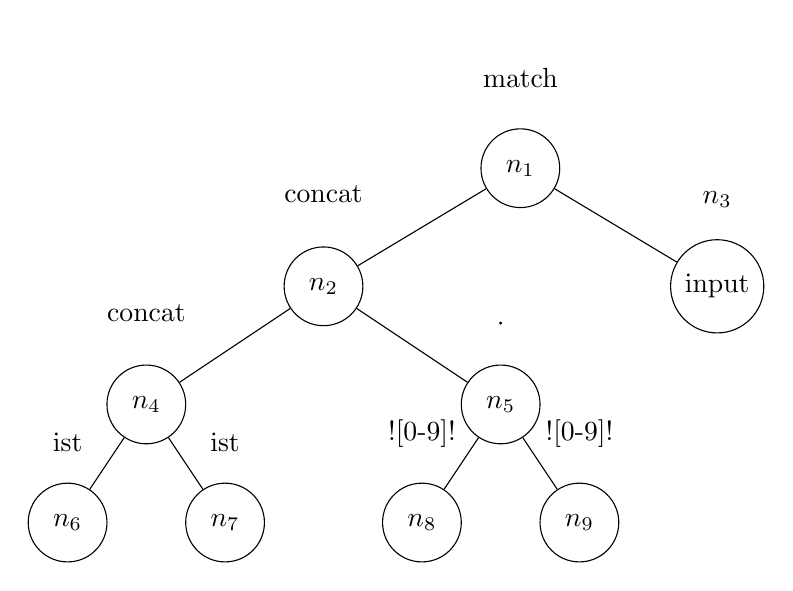
\begin{tikzpicture}[level distance=1.5cm,
level 1/.style={sibling distance=5cm},
level 2/.style={sibling distance=4.5cm},
level 3/.style={sibling distance=2cm}]
\tikzstyle{every node}=[circle,draw,minimum size=1cm]

\node (Root) [label={match}] {\(n_1\)}
child {
    node [label={concat}] {\(n_2\)} 
    child {
        node [label={concat}] {\(n_4\)}
        child { node [label={\regex{ist}}]{\(n_6\)} }
        child { node [label={\regex{ist}}]{\(n_7\)} } % edge from parent node[left, draw=none] {help!}
    }
    child {
        node [label={\(\boldsymbol{\cdot}\)}] {\(n_5\)}
        child { node [label={\Verb![0-9]!}] {\(n_8\)} }
        child { node [label={\Verb![0-9]!}] {\(n_9\)} }
    }
}
%
child {
    node [label={\(n_3\)}]{input}
};

\end{tikzpicture}
    \caption{Program tree for match validation with regular expression \regex{istist[0-9][0-9]}}
    \label{fig:example-regex-tree}
\end{figure}{}


\section{The first type of pruning things}

I was reading a fun book with a rose on its cover and it talked about 2 kinds of symmetries: solution symmetries and problem symmetries. (Obviously a hundred other authors gave these things a hundred other names, and this is how I know they are for real). I think this first kind of cool things correspond to the so-called problem symmetries. Anyway, these are the kind of pruning thing that are used to prevent the enumeration of programs that I know beforehand are unnecessary.

\subsection{Union is idempotent}
Union is an idempotent operation, i.e., for a regular expression, \(r\), the union of \(r\) with itself is \(r\) again:
%
\[r | r = r\]
%
Enumerating something of the type \(r|r\) is unnecessary. We could just write \(r\) which is obviously preferable. Therefore, we can just add constraints to prevent the enumeration of things like that one. It goes like so: if a node has a \textit{union} operation assigned to it, then ensure its subtrees are different. To ensure the subtrees are different, we simply have to state that one of the nodes in the subtree is different. Here, have an example:

\begin{figure}[t]
\centering
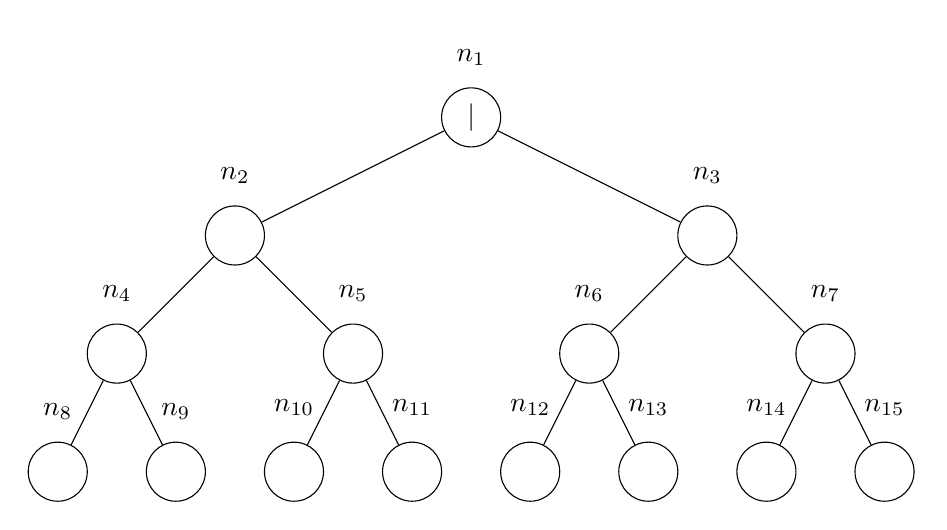
\begin{tikzpicture}[level distance=1.5cm,
level 1/.style={sibling distance=6cm},
level 2/.style={sibling distance=3cm},
level 3/.style={sibling distance=1.5cm}]
\tikzstyle{every node}=[circle,draw,minimum size=.75cm]

\node (Root) [label={\(n_1\)}] {\(|\)}
child {
    node [label={\(n_2\)}] {} 
    child {
        node [label={\(n_4\)}] {}
        child { node [label={\(n_8\)}]{} }
        child { node [label={\(n_9\)}]{} } % edge from parent node[left, draw=none] {help!}
    }
    child {
        node [label={\(n_5\)}] {}
        child { node [label={\(n_{10}\)}] {} }
        child { node [label={\(n_{11}\)}] {} }
    }
}
%
child {
    node [label={\(n_3\)}] {} 
    child {
        node [label={\(n_6\)}] {}
        child { node [label={\(n_{12}\)}]{} }
        child { node [label={\(n_{13}\)}]{} } % edge from parent node[left, draw=none] {help!}
    }
    child {
        node [label={\(n_7\)}] {}
        child { node [label={\(n_{14}\)}] {} }
        child { node [label={\(n_{15}\)}] {} }
    }
};

\end{tikzpicture}
    \caption{A part of a program which is a subtree of the original program tree. The root of this subtree has the \textit{union} operation assigned. }
    \label{fig:union-idempotent-tree}
\end{figure}{}


In \autoref{fig:union-idempotent-tree}, we have a tree which could be a bit of some program. The root of this subtree, here labelled \(n_1\) is a node who was assigned the operation \textbf{union}. Because of this, we want to ensure that the subtrees with roots \(n_2\) and \(n_3\) are different. To do this, we simply need to ensure that at least one of the nodes for one of the subtrees is different from the corresponding node from the other.

\[n_2 \ne n_3 \lor n_4 \ne n_6 \lor n_5 \ne n_7 \lor n_8 \ne n_{12} \lor n_9 \ne n_{13} \lor n_{10} \ne n_{14} \lor n_{11} \ne n_{15}\]

It prevents the enumeration of many unnecessary programs. And it makes it faster! Yay!!

\section{Kleene closure, positive closure and the question mark thing are idempotent}

\section{Positive closure and question mark do not make sense right after (or right before) a Kleene closure}

\[r^{*+} = r^{+*} = r^*\]
%
\[r^{*?} = r^{?*} = r^*\]
